% !TEX TS-program = pdflatexmk-c
\documentclass[11pt, letterpaper]{article}

\usepackage[brazilian, english]{babel}
\usepackage[utf8]{inputenc}
\usepackage[T1]{fontenc}
\usepackage[draft]{todonotes}   % notes showed
\usepackage{geometry}
\usepackage{lipsum}
\usepackage{enumitem}
\usepackage{float}
\usepackage{forest}


% set custom date and format
\usepackage[nodayofweek,level]{datetime}
\newcommand{\mydate}{\formatdate{17}{3}{2016}}
\newdateformat{mydateformat}{ \THEMONTH \dateseparator \THEDAY \dateseparator \THEYEAR}

\title{\vspace{-2cm} 19702 \\ Project 1}
\author{Francisco Fonseca \and Octavio Mesner}
\date{\mydate}

\date{\mydateformat\normalsize\mydate} % Today's date or a custom date

\begin{document}

\maketitle % Print the title

\section{Introduction} \label{intro}

New York City (NYC) would like to implement a fleet of autonomous
vehicles (AV) by 2020 as part of a larger initiative of establishing
itself as a world leader in smart city infrastructure. Because of the
novel nature of AV technology, there is a considerable amount of
uncertainty regarding the impact from its implementation on traffic
issues including
safety, congestion, energy consumption and environmental impacts.
City officials wish to determine the effect of each alternative, while
considering uncertainty, on these outcome
and optimal strategies moving forward with AV
technology within the NYC fleet of vehicles. This study will focus on
the alternatives available to implement  this technology
from AutoMerge, Inc. (AM) specifically in NYC's 40-passenger transit
buses. It will compare different alternative strategies by performing
a Benefit Cost Analysis (BCA) to assess how these different options
impact the general population of NYC, which are the main stakeholders
in this issue. Among the factors to be included in the analysis are:
safety, energy consumption, air pollution, GHG emissions, weather
conditions and traffic flow. Section \ref{problem} presents a detailed
description of the problem and the alternatives analyzed. Section
\ref{results} presents the analysis of each alternative and the
results found. In section \ref{sensitivity} a sensitivity analysis is
performed for some inputs. Section \ref{discussion} discusses the
results of the analyses and section \ref{conclusion} presents the
conclusion and recommendations of this study.

\section{Problem Description} \label{problem}
\subsection{Alternatives}

Broadly, NYC must consider the following three alternatives.

\begin{description}[leftmargin=0pt]
\item[Alternative 1:] Do not implement AV.

This is the reference alternative. AV is not implemented and the
benefits and costs are the ones already incurred to the population.
There is relatively little uncertanty associated with this outcome
because there is historical data to project the effect of this
alternative on outcomes.

\item[Alternative 2:] Implement AV in the NYC bus fleet.

In this alternative, the city implements the AV technology in the bus
fleet directly (without performing any pilot tests).  Because this is
an emerging technology, it is unclear how AV will perform in each
outcome so uncertainty analysis will help determine the expected value
for each outcome using the risk information currently available.

\item[Alternative 3:] Perform a pilot test with an amount of $n$ buses
  before deciding to implement AV.

In this alternative, the city performs a pilot test with a predefined
amount of $n$ buses. The pilot test has an associated cost directly
proportional to $n$.  The potential benefit of running a pilot study
is the additional information gained on risks associated with
congestion and other outcomes.  It will be necessary to calculate the
value of imperfect information for each $n$ for this alternative.

\end{description}

\subsection{Benefits, Costs \& Uncertainty}

Although public transit systems are essential to any urban area, they 
also incur several costs to the general population. Implementing AM 
in the bus system will impact these costs in different ways.

\begin{enumerate}[leftmargin=*]

\item \textbf{Capital and Operating Costs of implementing AM.}
  The most obvious costs are the capital and operating costs of implementing
  and operating the AM system in the buses. Ordinary capital and operating costs
  related to the bus operation will not be considered in this analysis since they
  will be incurred in all alternatives. Estimates for capital and O\&M costs for the AM 
  system were informed in a per bus basis, conditioned on the age of the bus. We 
  used this data to compute these costs.
  
  \begin{table}[h]
\caption{Capital and O\&M costs of the AM system}
\centering
\footnotesize
\renewcommand{\arraystretch}{1.1}
\begin{tabular}{c l l l}
\hline
 	& Variable 							& Value 				& Notes 						\\\hline\hline
(a)	& \# buses with age < 5 years				& 2313				& Source:						\\
(b)	& \# buses with age 5-9 years				& 1296				& Source:						\\
(c)	& \# buses with age 10-20 years			& 1437				& Source:						\\
(d)	& Capital Cost per bus age < 5 years		& \$ 5000				& Source:			\\
(e)	& Capital Cost per bus age 5-9 years		& \$ 6500				& Source:			\\
(f)	& Capital Cost per bus age 10-20 years		& \$ 8500				& Source:			\\
\textbf{(g)}	& \textbf{Total Capital Cost}(*)			& \textbf{\$ 45.7 Million}	& \textbf{=(a)*(d)+(b)*(e)+(c)*(f)}			\\
\\
(h)	& Annual O\&M Cost per Bus				& \$ 1500				& Source:		\\
\textbf{(i)}	& \textbf{Total Annual O\&M Cost} (**)	& \textbf{\$ 7.6 Million}	& \textbf{=[(a)+(b)+(c)]*(h)}			\\\hline\hline
\multicolumn{4}{l}{{\footnotesize (*) Capital costs are considered to be incurred only in the first year}} \\
\multicolumn{4}{l}{{\footnotesize (**) O\&M costs begin to occur in the fifth year of the analysis (when AM starts operating)}} \\
\end{tabular}
\label{tab:am.cost}
\end{table}%

  
\item \textbf{Traffic Congestion.}
  Being a part of the transit system, buses have an impact in the traffic congestion
  of NYC. This traffic congestion incurs in a social cost due to longer commutes, wasted hours for 
  the general population and additional fuel consumption. The use of AM can 
  have an impact in the traffic flow and potentially decrease these costs. To calculate 
  congestion costs, we only consider buses, cars, light duty vehicles, and trucks.  While walkers and
  cyclists do experience travel times, we do not believe that they
  will change with the different alternatives and do not need to be
  included for comparison purposes. Table \ref{tab:cong.cost} presents the computation of the 
  traffic cost for the reference case

\begin{table}[h]
\caption{Estimate of social costs due to traffic congestion in NYC}
\centering
\small
\renewcommand{\arraystretch}{1.1}
\begin{tabular}{c l l l}
\hline
 	& Variable 							& Value 				& Notes 						\\\hline\hline
(a)	& Annual Cost per Commuter				& \$ 300				& Source:						\\
(b)	& Annual hours in congestion per commuter	& 4 hours				& Source:			\\
(c)	& Cost per minute 						& \$ 13,400			& $(a)/[(b)*60]$		\\
(d)	& Total time person trip per day (*)			& 40,000 minutes		& Source: 						\\
\textbf{(e)}	& \textbf{Total annual congestion cost}	& \textbf{\$ 27 Million}	& \textbf{=360*(d)*(c)}			\\\hline\hline
\multicolumn{4}{l}{{\footnotesize (*) considers only Light Duty Vehicles, Motorcycles and Buses}}
\end{tabular}
\label{tab:cong.cost}
\end{table}%


\item \textbf{Fatalities \& Injuries.}  Another cost are traffic related injuries and fatalities. 
  Using AM in the bus system can have an impact in traffic safety and decrease these costs.
  The cost of each death is estimated using the standard Value of Statistical Life (VSL in \$). The 
  cost of each injury was estimated using data from CDC for injuries costs for each type of victim 
  (motorist, passenger, pedestrian, etc.). Using historical data of number of mortalities and injuries in 
  transit accidents in NYC ($N_{mort}$ and $N_{inj}$), we computed total cost of traffic mortalities 
  ($\mbox{Cost}_{mort}$) and injuries ($\mbox{Cost}_{inj}$).

\begin{table}[h]
\caption{Estimate of social costs due to traffic mortalities and injuries in NYC}
\centering
\small
\renewcommand{\arraystretch}{1.1}
\begin{tabular}{c l l l}
\hline
 	& Variable 							& Value 				& Notes 						\\\hline\hline
(a)	& VSL (2015 \$)						& \$ 9.2 Million			& Source:						\\
(b)	& Number of fatalities per year				& 4					& Source:			\\
\textbf{(e)}	& \textbf{Total annual mortality cost}	& \textbf{\$ 27 Million}	& \textbf{=360*(d)*(c)}			\\
\\
(c)	& Average Cost of Injury 					& \$ 13,400			& $=12*(a)*(P | U, 5\%, (b))$		\\
(d)	& Number of injuries per year				& 40,000				& Source: 						\\
\textbf{(e)}	& \textbf{Total annual injury cost}	& \textbf{\$ 27 Million}	& \textbf{=360*(d)*(c)}			\\\hline\hline
\multicolumn{4}{l}{{\footnotesize (*) considers only Light Duty Vehicles, Motorcycles and Buses}}
\end{tabular}
\label{tab:mortality.cost}
\end{table}%

\item \textbf{Emissions.}
  Another major external cost of the bus system is the one related to
  the emission of air pollution gases and greenhouse gases. These emissions result
  in major health hazards for the general population and can affect future climate. Implementing 
  AM can have an effect of changing these emissions by improving traffic flow. Because at this point 
  we have emission data available only for buses, we focused our emission cost estimate only on 
  buses. Emission factors for buses differ for when buses are in movement ($ef_m$ in g/mi) 
  and when buses are idle ($ef_{i}$ in g/min). Using these factors, the marginal cost of each type 
  of gas emission ($mc_g$ in \$/ton), the total vehicle travel time ($T$ in minutes), 
  the total vehicle distance ($D$ in miles) and an estimate of the share of travel time that 
  the vehicle is idle ($s_i$ in \%) we can compute total emission costs for each type of gas.

  \[\mbox{Cost}=\mbox{Cost}_{\mbox{run}}+\mbox{Cost}_{\mbox{idle}} = D \times ef_m \times mc_g +  s_i \times T \times  ef_i \times mc_g\]
  
  We assume that improvements from AM will only affect emissions as a result of idle time 
  (i.e., as congestion decreases, vehicles spend less time in idle status but still travel the same distance).
  
\end{enumerate}

In addition to the costs listed above, there are also uncertainties associated 
with the implementation of AM. One of the uncertain factor is what will be the effects
of AM in the congestion and safety of NYC transit system. Another source of 
uncertainty is how bad weather will affect the operation of the AM system. These two
types of uncertainty are included in our analysis.

\subsection{Assumptions}

\begin{enumerate}[leftmargin=*]
\item The number of riders using each mode of transportation will remain
  stable for all three alternatives.
\item Changes in congestion will affect motor vehicles (buses, cars,
  light duty vehicles, and trucks) but not bicycles or walkers.
\item All travel minutes across persons and modes of transportations
  are worth the same and includes fuel costs, \$22 per hour per individual.
\item Weather patterns remain consistent.
\item Any travel time, even fast ones, incurs a time cost.  This means
  that for each alternative, there will be a time cost added which is
  associated with it.
\end{enumerate}

\begin{table}[h]
\caption{General Assumptions}
\centering
\renewcommand{\arraystretch}{1.1}
\begin{tabular}{c l l l}
\hline
Variable 							& Value 				& Notes 			\\\hline\hline
Discount rate						& 5 \% per year			& Source:			\\
Time Horizon						& 20 years			& Source:			\\\hline
\end{tabular}
\label{tab:assumptions}
\end{table}%


\section{Methods}

For this analysis, we use a decision tree with standard expected
values to assess alternatives one and two and the value of imperfect
information to assess alternative 3.  Figure~\ref{decisiontree} shows
our decision tree for the first two alternatives.  This same paradigm
will be used to compute the expected value of imperfect information.

\begin{figure}[h]
\centering
\begin{forest}
for tree={grow=east}
[Decision
   [Alt 1[7,tier=word]]
   [Alt 2
      [Good Weather
         [MB[1,tier=word]][LB[2,tier=word]][LW[3,tier=word]]
      ]
      [Bad Weather
         [MB[4,tier=word]][LB[5,tier=word]][LW[6,tier=word]]
      ]
   ]
]
\end{forest}
\caption{Partial decision tree}\label{decisiontree}
\end{figure}

Each cost listed in Table \ref{tab:bca.costs} was estimated using data from different sources:

\section{Analysis and Results} \label{results}

%\todo[inline]{Write results.}

\subsection{Alternative 1: Don't Implement AV}

\subsection{Alternative 2: Implement AV}

\subsection{Alternative 3: Pilot test}

Figure \ref{fig:alt1} presents the resulting NPV for each alternative. For alternative 1 (reference case) we can observe that the component that results in the largest cost is air pollution. Total present value of costs is approximately \$ 31.4 Billion. Implementation of AM (alternative 2) results in a decrease of the expected present value of costs of approximately \$ 0.2 Billion or 0.7\%.

\begin{figure}[H]
\begin{center}
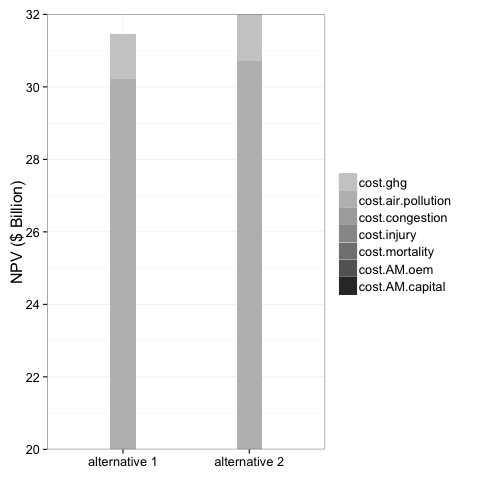
\includegraphics[width=0.45\textwidth]{../../R/barplot1}
\caption{Expected NPV (in Billion \$) computed for each alternative}
\label{fig:alt1}
\end{center}
\end{figure}

\section{Sensitivity Analysis} \label{sensitivity}

%\todo[inline]{Write sensitivity analysis.}

\section{Discussion} \label{discussion}

%\todo[inline]{Write discussion.}

\section{Conclusion \& Recommendations} \label{conclusion}

%\todo[inline]{Write Conclusion and Recommendations.}


\end{document}
